\documentclass[sigplan,screen]{acmart}
\AtBeginDocument{%`
  \providecommand\BibTeX{{%
    \normalfont B\kern-0.5em{\scshape i\kern-0.25em b}\kern-0.8em\TeX}}}

\begin{document}
\title{CS510 Project Report: Compression Approaches for Neural Ranking and Question Answering}
\author{Daniel Campos}
\email{dcampos3@illinois.edu}
\begin{abstract}
Neural Networks have proven to be effective methods for retrieving relevant document however these methods can prove difficult to use in production. Neural models tend to be large and require specialized hardware for inference(GPU, TPU, FPGA, etc) which makes them difficult to deploy for all use cases. Researchers in fields like computer vision have leveraged methods in model compression such as structured and unstructured pruning to decrease model size while preserving or exceeding original model performance. In our work we will explore the interplay between unstructured pruning, model distillation, and layer removal in relation to question answering and passage re ranking. In our experiments we find that     
\end{abstract}
\keywords{information retrieval, network pruning, question answering}
\maketitle

\section{Introduction}
Neural Networks have become popular choices for complex computation tasks like image recognition \cite{Howard2017MobileNetsEC}, image generation \cite{Goodfellow2014GenerativeAN}, speech processing \cite{Zhao2017RecurrentCN}, and question answering \cite{Seo2017BidirectionalAF} and ranking \cite{nogueira2019multi}. These networks have grown to hundred billions of parameters \cite{Brown2020LanguageMA} which require specialized hardware like clusters of GPUs and FPGAs in order to infer on unseen data.  In the world of Natural Language Processing (NLP) and information retrieval (IR), neural language model's adaptability and performance has made them popular model despite their size. In order to ensure advances in research have practical applications many researcher have explored how large neural models can be compressed. Methods  Recent work has shown that larger networks can learn quicker \cite{Li2020TrainLT}, are more accurate and are more sample efficient \cite{Kaplan2020ScalingLF} which will likely speed up adoption and drive scaling of neural models. As scaling laws will likley drive continue model growth methods of compression like quantization, distillation and pruning, are natural explorations points.  \\ 
Model distillation, quantization, and pruning have emerged as successful methods to produce smaller networks from the original over-parametized network. In model distillation \cite{Ba2014DoDN} the original network is used to train a smaller network to mimic the behavior of the large network. In model quantization \cite{Han2016DeepCC} models are made smaller by  reducing the numbers of bits that represent each weight. Model Pruning \cite{LeCun1989OptimalBD} has focused on finding sub-networks in the original network by structured and unstructured pruning. In structured pruning, successful sub-networks are found by removing neurons  \cite{Wang2019StructuredPF} or larger network specific structures like attention heads \cite{Voita2019AnalyzingMS}. In unstructured pruning the successful sub-networks are found by setting individual weights to zero \cite{Kwon2019StructuredCB}. With the introduction of transformer \cite{Vaswani2017AttentionIA} a simple compression method became normal, removal of transformer layers. Since methods like BERT rely on 12 and 24 stacked encoder layers it has become common that removal of encoding layers can be used to decrease the model size. Despite a wide exploration of these methods as applied to NLP, few methods have combined all three approaches and to the best of our knowledge there has been no explicit work focused on IR.\\
In our work we explore the intersection of unstructured pruning, model distillation, and layer dropping to generate the optimal compressed models for two IR tasks: Question Answering and Passage Ranking. While previous work on compressing question answering does exist \cite{Sanh2020MovementPA}, the work does not explore removal of layers, nor explore the effect of training length on pruning schedule. Moreover, despite the popularity of deep learning scale IR datasets like MSMARCO Passage Ranking (MPR) \cite{Campos2016MSMA}, no work has explored how compress-able these models are. Using these large scale datasets we find that question answering models can be pruned to 90 percent of their original weights, 50 \% of their layers removed and still keep close to the original performance. 
We believe the results of our work could motivate our future research and that of the broader IR community. 
The contributions of our work are as follows:
\begin{enumerate}
    \item Our work provides a exploration of the connection between distillation, network pruning, and layer removal for information retrieval tasks.
    \item Our work provides the first application of network pruning for passage retrieval
    \item Our Work provides the first exploration of training time as a factor in network pruning.
\end{enumerate}
\section{Related Work}
\subsection{Neural Rankers}
Like many computer science fields, Information Retrieval has seen neural network based systems out performing previous systems. Systems like DUET \cite{Mitra2017LearningTM}, DSSM \cite{Huang2013LearningDS}, C-KRNM \cite{10.1145/3159652.3159659}, and C-DSSM \cite{Shen2014LearningSR} leverage neural building blocks and classical IR ranking methodologies to produce results competitive with non neural methods. With the introduction of neural language models, countless BERT-based models produced new state of the art results similar to many other NLP fields \cite{nogueira2019multi}. Building on the success of the transformer and seeking to build document wide dependency modeling models leveraging the transformer such as Conformer-Kernel\cite{Mitra2020ConformerKernelWQ} have shown efficiency in quality and scale. In question answering, neural models have mirrored changes in ranking models. Approaches initially leveraged RNNs \cite{Shen2016ReasoNetLT,} \cite{Wang2017MachineCU} and quickly moved to include attention \cite{Seo2017BidirectionalAF} . With the introduction of BERT \cite{Devlin2019BERTPO}, improvement greatly improve and human performance was shortly outperformed.  
\subsection{Model Compression}
Neural network compression is an area that has attracted the attention of researchers for the last few decades. Methods for producing smaller networks that approximate original network performance include: distillation, quantization, structured and unstructured pruning. While each of these methods can compress models substantially on their own many researchers have found that some combination of these methods can produce the smallest models with the highest performance \cite{Polino2018ModelCV}, \cite{Sanh2020MovementPA}. \\
Model distillation \cite{Ba2014DoDN} addresses compressing models by first training a large network and calling it a teacher. Then using this teacher model a smaller student model learns to approximate what the teacher model would do. This framework is quite popular because it can leverage existing large models easily and the student model can be designed to fit the application requirements in terms of speed and model size. Distillation has been one of the most common methods of deployment of large scale language models where student models like DistilBERT \cite{Sanh2019DistilBERTAD} can approximate full model performance at a fraction of the size. \\
Model quantization \cite{Gong2014CompressingDC} \cite{Han2016DeepCC} addresses compressing models by reducing the number of bits that are require to represent parameters in a model. In simple implementations this means changing representation of weights from Float32 to float16(effectively cutting model size in half). Complex implementations tune networks to find the smallest amount of bits that can be used for weights, biases, and gradient updates using values as low as 1 bit \cite{Courbariaux2016BinarizedNN}. Quantization is particularly effective because it both leverages that networks are defaulted to a level of precision which is too high and by decreasing the size of representations networks are forced to share weights making networks more robust. \\
Model pruning \cite{LeCun1989OptimalBD} addresses model compression by decreasing the connection in a network. The goal of network pruning is to produce a sub network of the original network which optimizes some network property(accuracy, speed, robustness) while preserving the original network function. Network pruning has been show to produce a similar effect to random noise injection \cite{Bartoldson2019TheGT} and this noise can be used to make the network more efficient. Bartoldson et al., showed that network pruning is not just used for decreasing size but can be used to increase the generalization of the network. 
As mentioned earlier, there is structured pruning and unstructured pruning. In structured pruning, the structure of the network is altered by removal of entire neurons, layers, or portions neural network. This method has proven especially successful in language model compression where despite having dozens of attention heads \cite{Vaswani2017AttentionIA} few heads do most of the work and the rest can be removed \cite{Michel2019AreSH}. In unstructured pruning the network structure is altered by removal of individual weights. Unstructured pruning when paired with optimization engines can produce networks that are smaller, more accurate, and run faster than the original network. \\
\section{Method}
To evaluate the effect of method compression we will explore how the combination of said methods effects two Information Retrieval tasks: Question Answering and Passage Retrieval. For each of the aforementioned tasks, we train tasks specific models built on bert-base-uncased. Given this baseline, we proceed to train variants with layers removed, with distillation, and with various degrees of unstructured pruning.
\subsection{Question Answering}
Question answering is the goal of providing an answer to a query $q$ given some sort of context passage $p$. While there are abstractive methods because of difficulty in evaluation we will focus on extractive methods. Extractive systems predict two attributes for each query and context passage: $token_{start}$ and $token_{end}$ each of which denotes an token index in a context passage. As a result, the answer $a$ to a query $q$ is $a=\{t_{token_{start}},...,t_{token_{end}}\}$. \\
The \textbf{S}tanford \textbf{QU}estion \textbf{A}nswering \textbf{D}ataset 1.1 (SQUAD) dataset has become the standard for extractive question answering. Constructed out of 500 context passages derived from Wikipedia it contains 100,000+ question-answer where each question was written by a human annotator. While there have been updates to the dataset and additional question answering datasets the widespread use of SQUAD makes it a logical choice. \\
\subsection{Passage Re-Ranking}
Passage ranking is a task which seeks to provide relevant short context passages for a given user query. These systems are commonly used as first stage retrievers for con question answering models. Since passages tend to have short context windows (under 512 tokens) transformer \cite{Vaswani2017AttentionIA} have become efficient models. With the introduction of large scale ranking datasets like MSMARCO \cite{Campos2016MSMA} and ODQA \cite{Karpukhin2020DensePR} data hungry neural methods thrived. Passage Retrieval has three main formulations, sparse retrieval,  dense retrieval, and hybrid retrieval. Sparse retrieval leverages traditional retrieval mechanisms like BM25 to rank relevant candidates. Dense retrieval leverages encoders which map queries and passages to a shared vector space and ranks candidates using an Approximate Nearest Neighbor index. Hybrid retrieval focuses on some combination of dense retrieval and commonly includes a sparse 1st stage ranker followed by a dense re-ranker. Our work focuses on Hybrid Retrieval on the MSMARCO Passage Retrieval dataset.\\
The MSMARCO dataset was originally a 1,000,000+ sample question answering dataset where given 10 context passages $p$, a human judge selected the most relevant passage and wrote the answer. This dataset was re-purposed for passage ranking by creating a collection of all unique passages and evaluating candidates ranking ability. Since the corpus does not contain a definitive ranking to optimize models train using negative and positive examples of query-passage relevance. Since relevance labels are binary, we follow standard training procedures and treat the task as a binary classification task. Given a query $q$ and a passage $p$ a model predicts how likely this pair is to belong in the relevant class. 
\subsection{Distillation}
Distillation can be considered an effective method for label smoothing \cite{Hinton2015DistillingTK}. Our focus is on self distillation where a teacher model is used to distill its learning into a student model. The teacher model is trained to convergence using cross entropy loss while the student is trained with a combination of the cross entropy loss and the Kullback–Leibler divergence between the student and teacher logits. Cross entropy is represented in equation \ref{cross}, and the distillation loss is shown in equation \ref{distill} where $sl$ are student logits, $tl$ are teacher logits, $\lambda$ is a distillation hardness,and $KL$ is the Kullback–Leibler divergence. 
\begin{equation}
L_{crossentropy} = - \sum_{i} ({y_i' \log(y_i) + (1-y_i') \log (1-y_i)})
\label{cross}
\end{equation}
\begin{equation}
L_{distill} = (1- \lambda )(L_{crossentropy}) + \lambda (KL(sl, tl))
\label{distill}
\end{equation}
\subsection{Compression}
Our work explores compression via unstructured pruning and layer removal. Language models like BERT are created by stacking identical layers of transformers and as a result compression can be achieved by simply removing these layers. We assign a mapping of layers to keep given target network depth based on experiments on most efficient methodologies and we find that for 1 layer networks we keep the first layer, for 3 we keep 1,6,12, for 6 we keep odd layers(1,3,5,7,9,11), for 9 we keep 1,3,4,5,7,8,9,10,12.
Unstructured pruning is the removal of weights in a network until a desired amount of weights remain. This is commonly achieved by setting weights in a network to zero or by adding a mask on top of network weights. Our work focuses on the the gradual removal of weight which have the smallest magnitude (magnitude pruning). Network layers are pruned independently of each other meaning that all components in a network share sparsity levels. Pruning is implement using Neural Magic's \footnote{https://neuralmagic.com/} sparseML library which introduces configurable sparsity in models with minimal overhead. \\
Layer removal is perhaps the simplest method we study as it solely focus on removing layers from a language model. Language models like BERT are created by stacking identical layers of transformers and as a result compression can be achieved by simply removing these layers. 
\section{Experiment}
For each of our experiments we  use the bert-base-uncased BERT model. It has 109m parameters and consists of 12 transformer layers with 768 hidden dimensions, 12 attention heads and a sub word vocabulary of 30,522 tokens. We choose this model because of its success across NLP and question answering, and information retrieval. For ease of reproduction we have build all of our experiments using Hugging Face's Transformers and network pruning was implemented using Neural Magic's sparseml.
\subsection{Question Answering}
For question answering we train using mostly fixed hyperparamets where batch size is 16, learning rate is 3e-5 and we leverage adamW , max sequence length is 384, and all training is done using float16. Models are kept fixed except for train length and any layers that are removed. When we explore removing layers they are removed prior to training and follow the structure described in method. Our baseline matches previously reported results and is achieved in 2 epochs. Our teacher model for distillation is our sparse baseline and after manual experimentation we find a distill hardness of $\lambda=1$ and temperature=2 to be optimal. \\
Our first experiments shown in table \ref{tab:qa-prune-length} show that high sparsity models can retain model performance but training length has to be extended substantially. Our experiments also find that no sparsity is able to support zero shot pruning as this causes huge variations in end model performance (up to 30 absolute F1 percentages). 
\begin{table}[b]
\resizebox{8cm}{!}{
\begin{tabular}{|l|l|l|l|l|l|l|}
\hline
sparsity   & total epochs      & pruned   & one shot   & pruning epochs & F1  & EM\\ \hline
0          & 1                       & no        & no         & 0              & 84.57     & 76.04\\ \hline
0          & 2                       & no        & no         & 0              & 88.02     & 80.63\\ \hline
0          & 10                      & no        & no         & 0              & 87.60     & 79.13\\ \hline
80         & 1                       & yes       & yes        & 0              & 25.14     & 15.10\\ \hline
80         & 2                       & yes       & no         & 0              & 66.96     & 53.88\\ \hline
80         & 10                      & yes       & no         & 8              & 83.95     & 74.41\\ \hline
80         & 30                      & yes       & no         & 18             & 84.06     & 74.64\\ \hline
90         & 1                       & yes       & yes        & 0              & 16.06     & 07.79\\ \hline
90         & 2                       & yes       & no         & 0              & 64.19     & 50.95\\ \hline
90         & 10                      & yes       & no         & 8              & 79.09     & 68.18\\ \hline
90         & 30                      & yes       & no         & 18             & 79.65     & 68.51\\ \hline
95         & 1                       & yes       & yes        & 0              & 10.50     & 04.93\\ \hline
95         & 2                       & yes       & no         & 0              & 24.45     & 14.44\\ \hline
95         & 10                      & yes       & no         & 8              & 72.76     & 60.41\\ \hline
97         & 10                      & yes       & no         & 6              & 70.26     & 57.02\\ \hline
97         & 30                      & yes       & no         & 18             & 70.43   & 57.29\\ \hline
99         & 1                       & yes       & yes        & 0              & 09.69     & 03.61\\ \hline
99         & 2                       & yes       & no         & 0              & 17.43     & 07.87\\ \hline
99         & 10                      & yes       & no         & 8              & 47.31     & 32.56\\ \hline
\end{tabular}}
\caption{Effect of pruning length at various sparsity's for question answering. Short pruning schedules produce irregular results while long pruning schedules produce minor drops in accuracy}
\label{tab:qa-prune-length}
\end{table}
\begin{table}[]
\resizebox{8cm}{!}{
\begin{tabular}{|l|l|l|l|l|l|l|l|}
\hline
sparsity   & params                  & Distilled & pruned   & layers     & pruning epochs & F1 Score   & EM Score  \\ \hline
0          & 108,893,186             & no        & no        & 12         & 0              & 88.00     & 80.63\\ \hline
0          & 108,893,186             & yes       & no        & 12         & 0              & 89.02   & 82.03  \\ \hline
0          & 87,629,570              & no        & no        & 9          & 0              & 86.70   & 78.82  \\ \hline
0          & 87,629,570              & yes       & no        & 9          & 0              & 87.94   & 80.46  \\ \hline
0          & 66,365,954              & no        & no        & 6          & 0              & 81.64   & 72.67  \\ \hline
0          & 66,365,954              & yes       & no        & 6          & 0              & 83.46   & 75.03  \\ \hline
0          & 45,102,338              & no        & no        & 3          & 0              & 51.75   & 39.11  \\ \hline
0          & 45,102,338              & yes       & no        & 3          & 0              & 43.83   & 33.06  \\ \hline
0          & 30,926,594              & no        & no        & 1          & 0              & 26.23   & 17.32  \\ \hline
0          & 30,926,594              & yes       & no        & 1          & 0              & 28.10   & 18.50  \\ \hline
20         & 108,893,186             & no        & yes       & 12         & 18             & 87.20   & 79.17  \\ \hline
20         & 108,893,186             & yes       & yes       & 12         & 18             & 89.56   & 82.74  \\ \hline
40         & 108,893,186             & no        & yes       & 12         & 18             & 86.27   & 78.08  \\ \hline
40         & 108,893,186             & yes       & yes       & 12         & 18             & 89.77   & 83.06  \\ \hline
60         & 108,893,186             & no        & yes       & 12         & 18             & 86.44   & 77.95  \\ \hline
60         & 108,893,186             & yes       & yes       & 12         & 18             & 89.38   & 82.29  \\ \hline
72         & 108,893,186             & no        & yes       & 12         & 18             & 85.50   & 76.43  \\ \hline
72         & 108,893,186             & yes       & yes       & 12         & 18             & 89.11   & 83.04  \\ \hline
80         & 108,893,186            & no        & no        & 12           & 18             & 84.06   & 74.64\\ \hline
80         & 108,893,186            & yes       & yes       & 12           & 18             & 88.03   & 80.81\\ \hline
80         & 66,365,954              & no        & yes       & 6          & 18             & 77.87   & 67.08  \\ \hline
80         & 66,365,954              & yes       & yes       & 6          & 18             & 84.69   & 76.57  \\ \hline
90         & 108,893,186            & no        & no        & 12           & 18             & 79.65   & 68.51\\ \hline
90         & 108,893,186            & yes       & yes       & 12           & 18             & 85.63   & 77.41\\ \hline
90         & 66,365,954              & no        & yes       & 6          & 18             & 73.52   & 61.22  \\ \hline
90         & 66,365,954              & yes       & yes       & 6          & 18             & 80.54   & 71.00  \\ \hline
97         & 108,893,186            & no        & no        & 12           & 18             & 70.43   & 57.29\\ \hline
97         & 108,893,186            & yes       & yes       & 12           & 18             & 75.013   & 63.95\\ \hline
97         & 66,365,954              & no        & yes       & 6          & 18             & 67.27   & 53.86  \\ \hline
97         & 66,365,954              & yes       & yes       & 6          & 18             & 72.36   & 60.82  \\ \hline
\end{tabular}}
\caption{Effect of layer dropping, distillation, and pruning on question answering BERT.}
\label{tab:qa-all}
\end{table}
\begin{figure}[h]
\centering
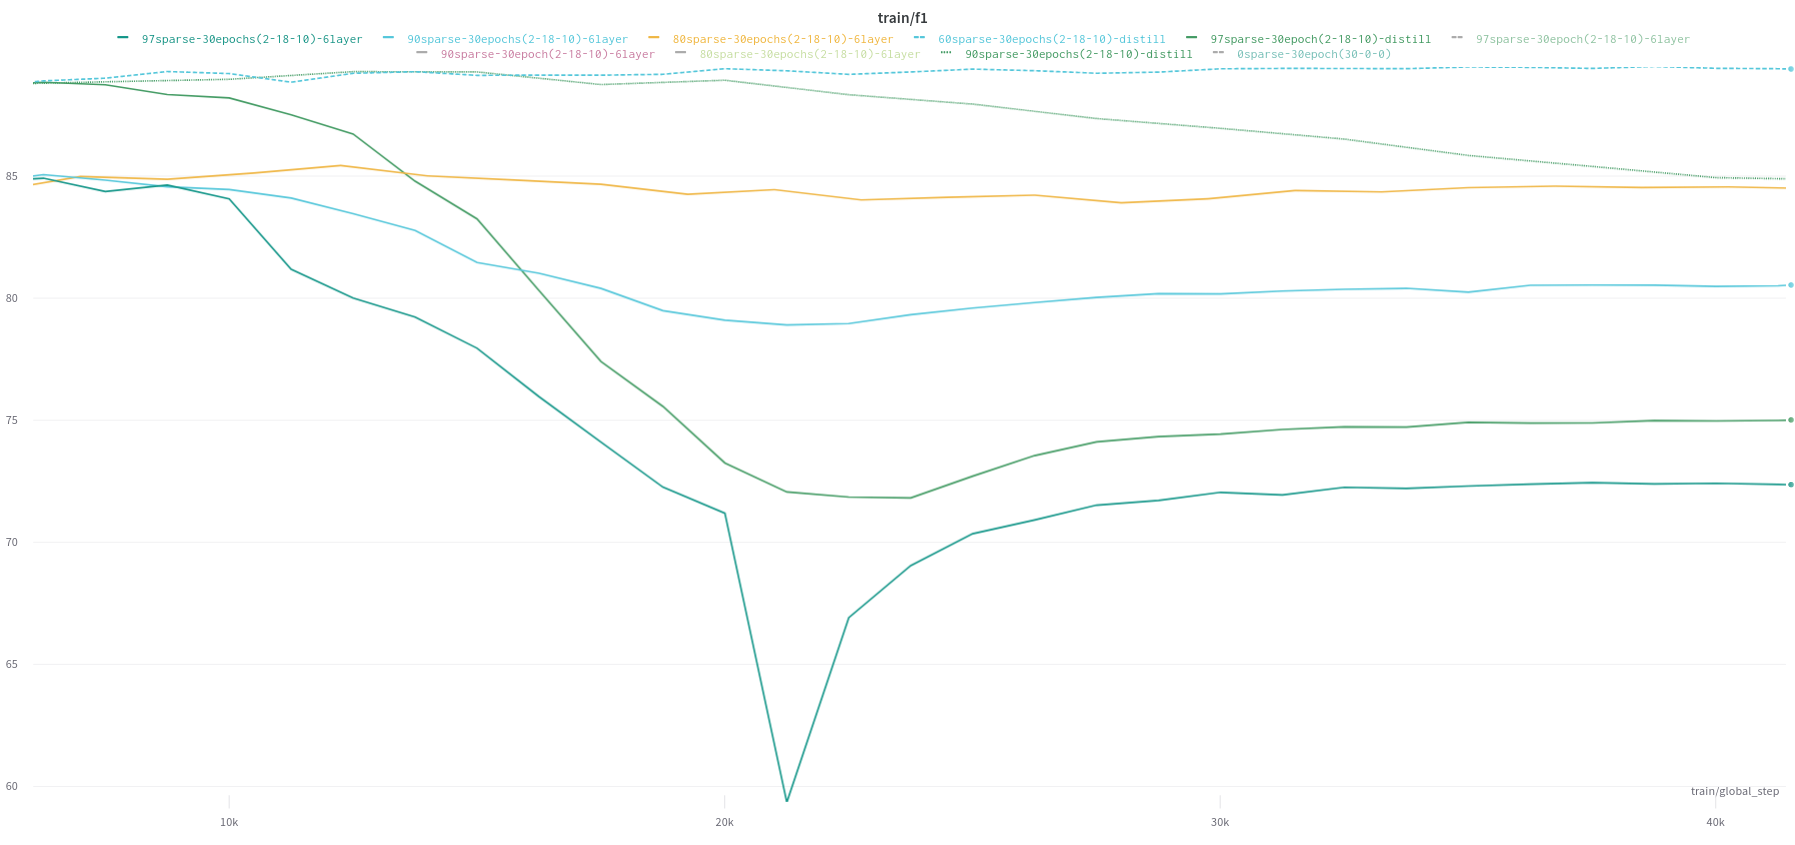
\includegraphics[width=8cm]{project/qaf1.png}
\caption{F1 Variations across question answering compressed models variants over training.}
\end{figure}
\begin{figure}[h]
\centering
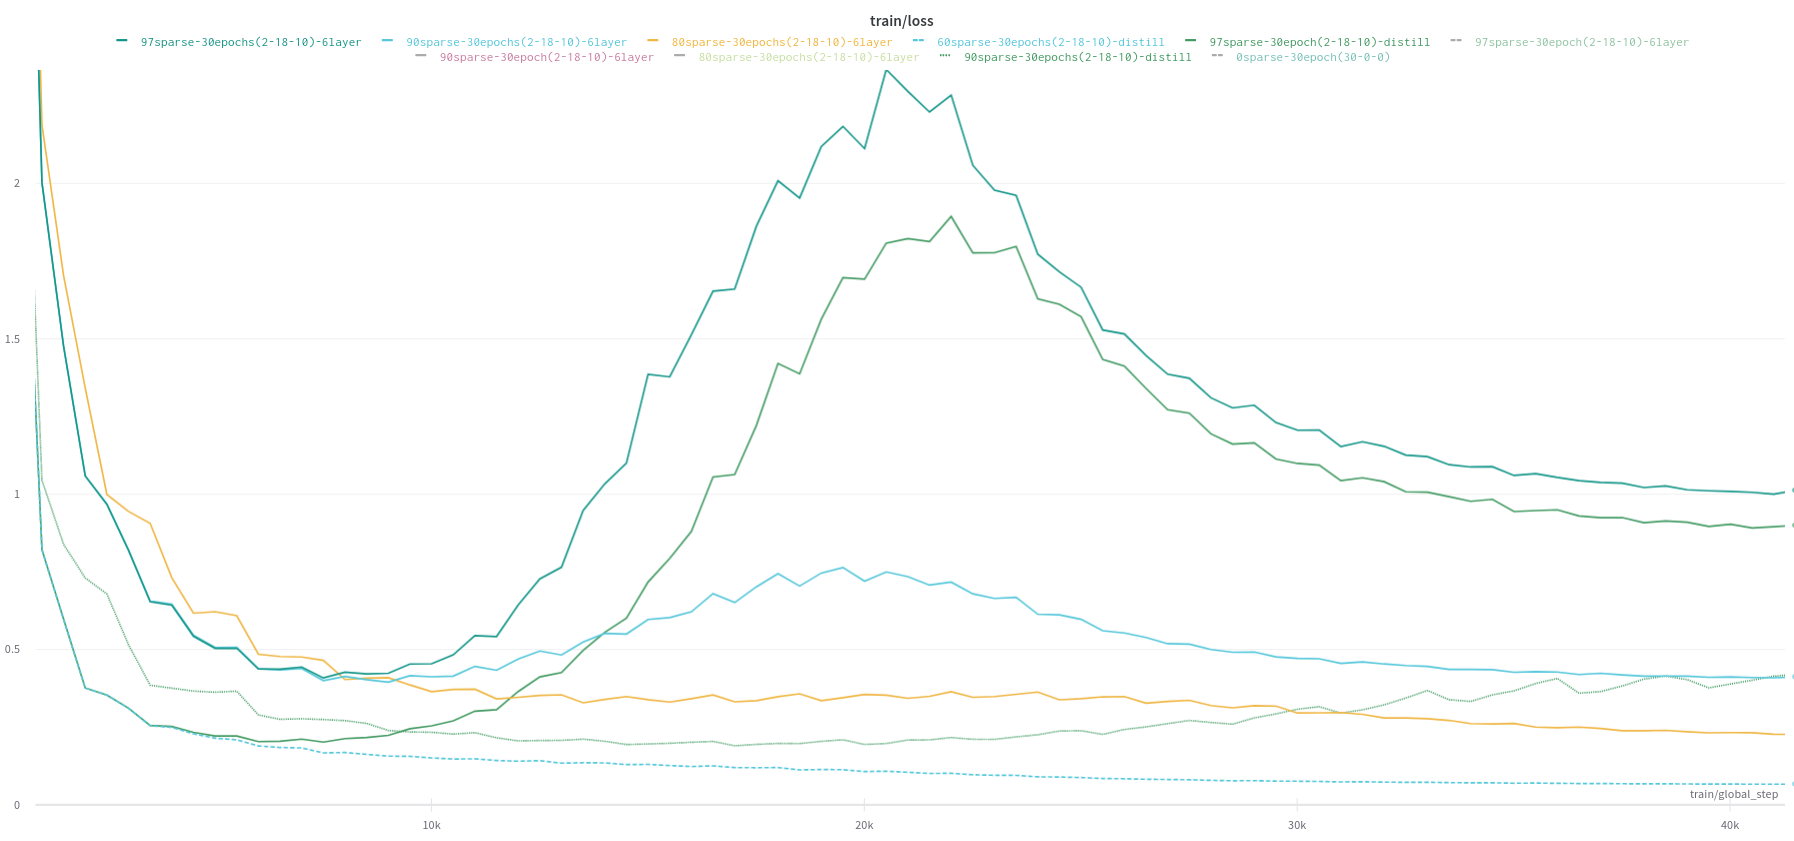
\includegraphics[width=8cm]{project/qaloss.png}
\caption{Loss Variations across question answering compressed models variants over training.}
\end{figure}
Our experiment also find that the relative reduction in parameters caused by layer removal is far more detrimental than network pruning. A distilled model with 72 \% sparsity has about the same amount of parameters as a 3 layer model but its performance is over twice as good and even better than the baseline. We believe this is strong supporter of the effects of sparsity and model distillation as a training regularizer. Our final result show a model with only 2\% active weights only sees a 16 point drop in quality(97\% sparse, 6 layer, distilled) and a 80 sparse, distilled 6 layer model is only 4\% worse than the baseline. On a current state of the art NVIDIA V100 16GB GPU each sample takes 12.77ms \footnote{https://github.com/NVIDIA/DeepLearningExamples/blob/master/TensorFlow/LanguageModeling/BERT/README.md}. When we our sparse models with efficient inference engines like Deepsparse can achieve equal accuracy with 41.19ms/sample on a commodity CPU!
\subsection{Passage Ranking}
Our Approach for passage ranking mirrors our experiments for question answer with minor tweaks to account for the MSMARCO corpus. We update the batch size to 64 and max sequence length to 128. Since the training corpus is ~80m samples, we stop training when loss stops improving. As inference is expensive we do not perform relevance evaluation on each of the 8.8m passages for each query. We use a first stage BM25 model to retrieve and rank the 1000 most relevant pass sage and then re rank those items.  Models are kept fixed except for sparsity, distillation, and layer that are removal. When we explore removing layers they are removed prior to training and follow the structure described in method. \\
As the MSMARCO dataset is over 800,000,000 training examples training on the full dataset is not feasible. Moreover, in long training experiments we do not find any improvement in loss or ranking ability after 1\% of the data is seen. Experiments with distillation found distillation less effective but best results come from a distill hardness of $\lambda=1$ and temperature=2. Experiments with pruning follow findings with our QA pruning experiments and train for 10x as long. It is worth noting that while our re-ranking method outperforms BM25, it does not perform as well as the methods on the MSMARCO leaderboard and are unsure as to why. We experimented with other mixtures of data selection like negative random sampling and negative samples being another positive sample but these dataset provided worse results than the existing MSMARCO dataset. As we could not improve model scores, we focus our efforts on the change with induced sparsity.  \\
The MSMARCO passage ranking dataset has a development set of 6800 queries. For evaluation we follow other work on the dataset and use mean reciprocal rank (MRR) at depth 10 and also study recall at the same depth. For our baseline, we use the public MSMARCO baseline BM25 implementation. As evaluation on this entire dataset takes over 6 hours (6.8 m query url pairs to predict relevance on), we run all of our experiments on a subset of 500 queries as we found that at this size, volatility in metrics is low.\\
Looking at the results shown in table \ref{msmarco} we see that the results are very different than seen in question answering. In passage ranking, model performance does not seem to be heavily tied to model size. Variations in layer removal or pruning rate only have minor degradation's in performance if any. Additionally, unlike question answering, distillation tends to have a negative effect. This is in line with our expectations as the MSMARCO labels are binary and as a result any form of label smoothing is much less important than on probabilities in 384 token context window. Finally, unlike question answering, pruned IR models perform substantially worse despite distillation. It seems that the IR model has learned a ranking function that is more dependent on in layer relations than multi layer transformation. We believe this is interesting because if follows some of the work of other researchers with single layer transformer models. \\
While our results do not point to large differences in performance for compressed passage ranking, we believe this is more of a factor of our model never learning a good representation for the data. Performance for our model is over 30\% worse than some of the other BERT models and as a result model degradation may not be visible as the models have not learned the task well. 
\begin{table}[h]
\resizebox{8cm}{!}{
\begin{tabular}{|l|l|l|l|l|l|}
\hline
sparsity   & distill & layers   & parameters  & MRR@10 & Recall @10\\ \hline
BM25       & no      & N/A      & N/A         & 0.167  & 0.558 \\ \hline 
0          & no      & 12       & 108,893,186 & 0.215  & 0.417 \\ \hline
0          & yes     & 12       & 108,893,186 & 0.213  & 0.427 \\ \hline
0          & no      & 9        & 87,629,570  & 0.208  & 0.397 \\ \hline
0          & no      & 6        & 66,365,954  & 0.208  & 0.397 \\ \hline
0          & no      & 3        & 45,102,338  & 0.207  & 0.395 \\ \hline
0          & no      & 1        & 30,926,594  & 0.207  & 0.395 \\ \hline
80         & no      & 12       & 108,893,186 & 0.199  & 0.403 \\ \hline
80         & yes     & 12       & 108,893,186 & 0.001  & 0.001 \\ \hline
80         & no      & 6        & 66,365,954  & 0.190  & 0.401 \\ \hline
80         & yes     & 6        & 66,365,954  & 0.003  & 0.018 \\ \hline
90         & no      & 12       & 108,893,186 & 0.157  & 0.353 \\ \hline
90         & yes     & 12       & 108,893,186 & 0.001  & 0.002 \\ \hline
90         & no      & 6        & 66,365,954  & 0.179  & 0.367 \\ \hline
90         & yes     & 6        & 66,365,954  & 0.005  & 0.016 \\ \hline
97         & no      & 12       & 108,893,186 & 0.101  & 0.251 \\ \hline
97         & yes     & 12       & 108,893,186 & 0.001  & 0.004 \\ \hline
97         & no      & 6        & 66,365,954  & 0.014  & 0.335 \\ \hline
97         & yes     & 6        & 66,365,954  & 0.003  & 0.016 \\ \hline
\end{tabular}}
\caption{Effect of pruning length at various sparsity's for passage ranking. Removal of layers does not heavily effect performance pruning, distillation and a combination of the three do.}
\label{tab:msmarco}
\end{table}
\begin{figure}[h]
\centering
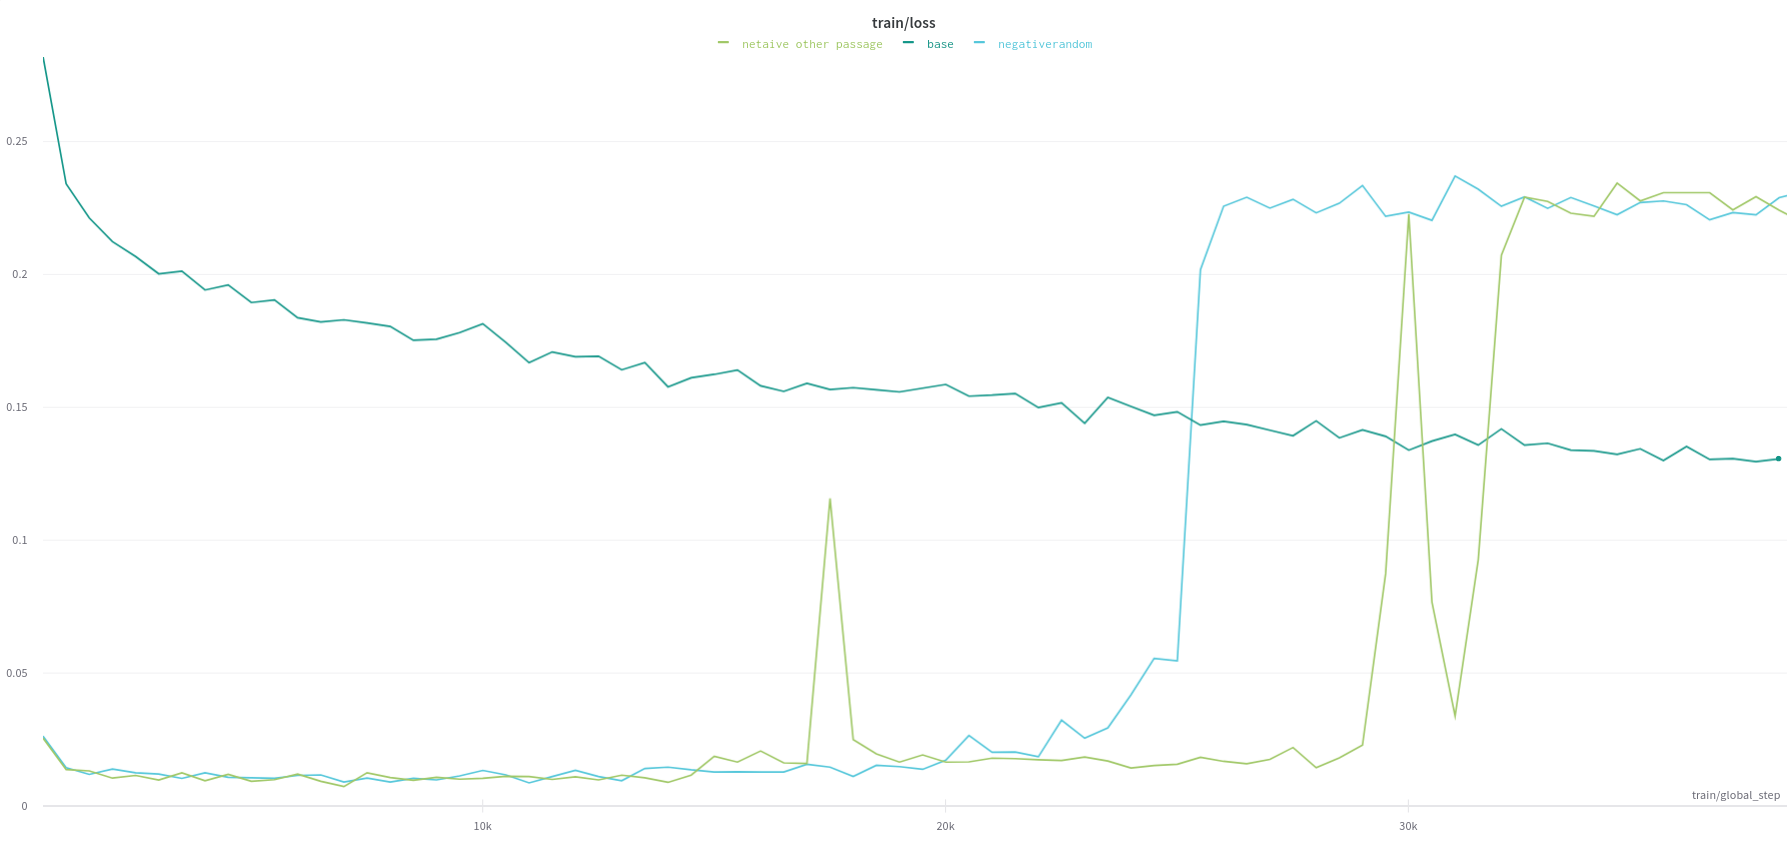
\includegraphics[width=8cm]{project/prunecurves.png}
\caption{Loss Variations across Passage ranking training corpora.}
\end{figure}
\section{Conclusion}
In our experiment we have shown that model distillation, layer dropping, and unstructured pruning are all powerful methods which can be used to make models substantially smaller without major accuracy losses. When focused on question answering, we are able to produce models that have less than 4\% decrease in performance despite being $\frac{1}{8}$ of the original size. Unlike previous methods exploring pruning for question answering, we are able to extract better results by enforcing uniform sparsity and leveraging GMP and long training regimes. Moreover, we showed that when knowledge distillation is employed, moderate pruning (40\%-70\%) can serve as a regularizer which helps the network out perform its original self. When focused on information Passage Ranking, the answer is less definitive. 
\section{Future Work}
In the future we wish to continue this work on model compression in information retrieval but will focus on Dense Passage Retrieval (DPR) \cite{Karpukhin2020DensePR} based methods. We believe these methods are of interest because compression of Siamese (Query encoder and document encoder) have not deeply studied. Given the success we saw in model size and even performance with pruning and distillation we believe we will likely find similar patterns with dual networks and we can use that to speed up index generation time. Currently, with a 20 million passage corpus DPR methods take 9 hours on a machine with 8 V100 GPUs for encoding and another 9 for indexing. With compression methods we believe we can likely cut that time in half. This is still orders of magnitude off of the Lucene sparse index generation which takes approximately 2 minutes. 
\section{Challenges}
This research project generally had two problems, performance replication and compute constraints. Replication performance lies in our inability to reproduce results cited by others in previous work and only plagued our experiments on the MSMARCO Passage Ranking corpus. Despite hours of tweaking the dataset, ranking methods, and broad hyperparameter sweeps, our best non-compressed experiment is far worse than methods in the literature. This was difficult because we spent a large portion of time trying to explore where failures may be and how to alleviate them instead of exploring a broader space of system compression. Our second challenge, compute, is a perpetual problem and has few solutions. Compression methodologies currently require many experiments with extended train times on large GPU clusters. Especially in the MSMARCO dataset where evaluation on the full validation set takes over 6 hours research cycles are slow. In order to deal with this problem we kept re adjusting project scope based on computational availability.  
\bibliographystyle{ACM-Reference-Format}
\bibliography{bibliography}
\end{document}
\endinput

